\section{Clock Drift}

The Tmote Sky uses a MSP430 microcontroller clocked an integrated ring oscillator called the Digitally Controlled Oscillator (DCO).
Since the generated clock frequency varies with temperature, voltage and from chip-to-chip, the DCO can be fine-tuned using a modulation functionality.
During booting, TinyOS calibrates the DCO using the external low-current 32.756Hz watch crystal to generate a more accurate 1MHz clock.
It should be noted, that calibration only accurs after a reset, and not periodically during program execution.

We noticed a problem, were serial communication stopped working after heating the nodes above $55-60\,^{\circ}\mathrm{C}$. Below this temperature the problem could be mitigated by resetting the mote to trigger a recalibration of the DCO.
We therefore looked at the output of the UART module with a logic analyzer and measured the how the selected baudrate changes over temperature.
Since the baudrate is generated by scaling the DCO, relative baudrate error is equivalent to relative DCO error.
Figure~\ref{fig:baudrate_error} shows the relative error of four baudrates over temperature.
We calculate an average temperature clock drift coefficient of $-0.367\%/\,^{\circ}\mathrm{C}$, which is within the typical range according to the datasheet. Similar coefficients were found by Z{\'u}{\~n}iga~\etal~\cite{Zuniga2013}.

\begin{figure}[ht]
	\subfigure[Relative error of four baudrates.] {
    	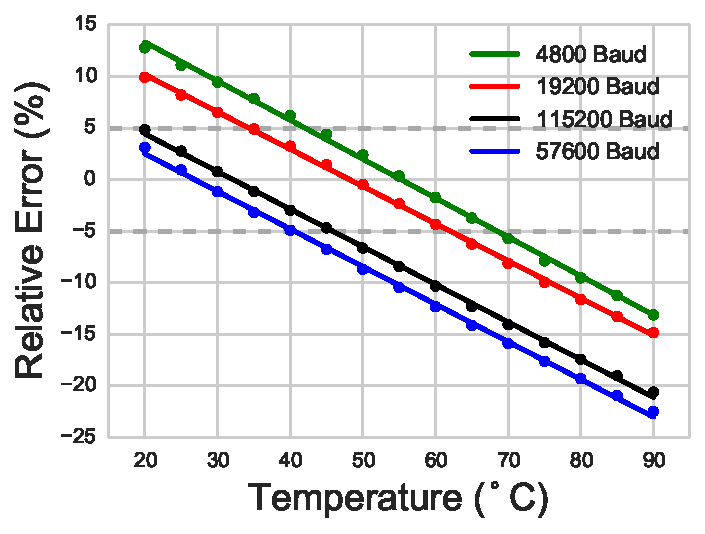
\includegraphics[width=0.5\columnwidth]{figures/baudrate_error}
    	\label{fig:baudrate_error}
    }
    \subfigure[Relative error of DCO calibration.] {
	    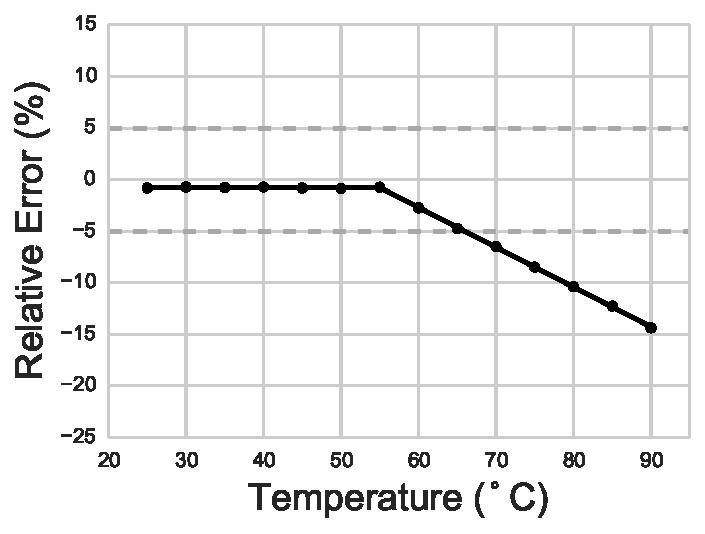
\includegraphics[width=0.5\columnwidth]{figures/reboot_dco_drift}
	    \label{fig:reboot_drift}
	}
	\subfigure[Relative error of corrected baudrate.] {
	    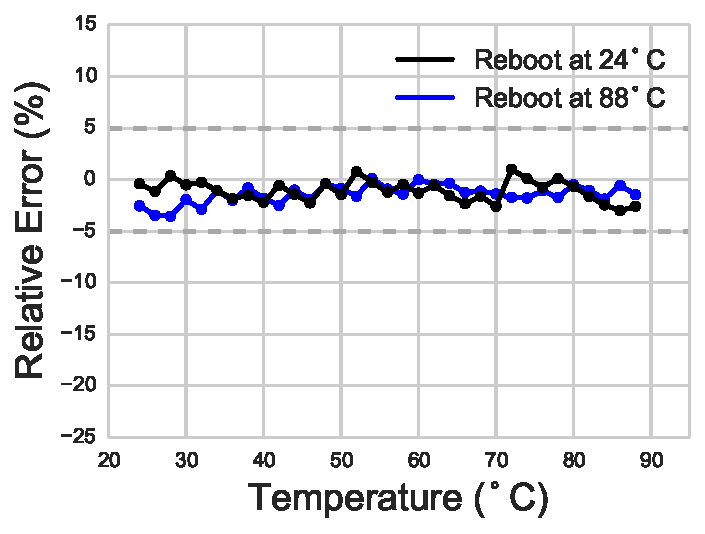
\includegraphics[width=0.5\columnwidth]{figures/baudrate_correction_error}
	    \label{fig:baudrate_look_up_error}
	}
	\subfigure[Values of baudrate correction look-up table.] {
	    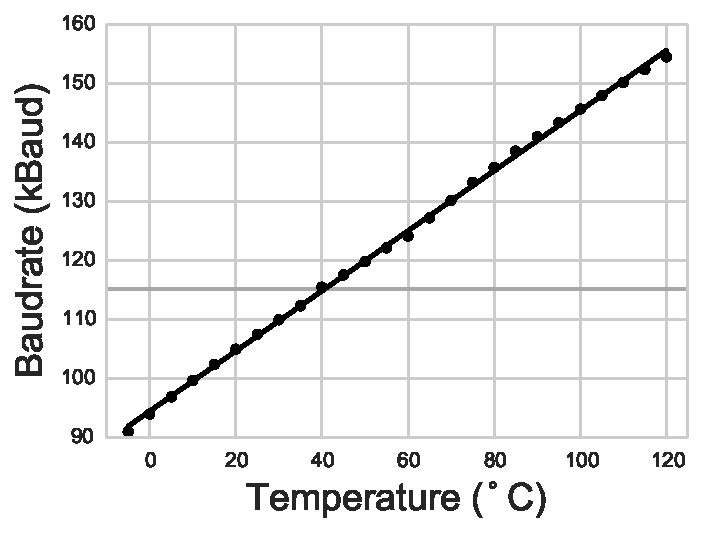
\includegraphics[width=0.5\columnwidth]{figures/baudrate_correction_table}
	    \label{fig:baudrate_look_up}
	}
	\caption{UART and DCO calibration errors vs. temperature. Note that UART can tolerate up to $\pm5\%$ error.}
\end{figure}

We then measured the relative baudrate error after rebooting over temperature.
As shown in Figure~\ref{fig:reboot_drift}, the TinyOS implementation of the DCO calibration only works until $55\,^{\circ}\mathrm{C}$, after which it has no corrective effect on CPU frequency, making periodic DCO calibration during program execution ineffective.

We chose not to correct clock drift directly, but counteract the effect on baudrate, by creating a lookup-table of ``inverse'' correction baudrates for 115.2kbps and applying it with temperature as shown in Figure~\ref{fig:baudrate_look_up}.
Since calculation of prescaler values at runtime is costly, the look-up table contains precalculated values, which are then copied into the registers at runtime.
The on-board sensor provides temperature to the UART module which then selects new prescaler values from the look-up table for every $5\,^{\circ}\mathrm{C}$, which shows as a sawtooth pattern in the resulting relative error of the corrected baudrate as shown in Figure~\ref{fig:baudrate_look_up_error}.

Note that the receiver can still correctly read serial data if the relative error does not deviate more than $\pm5\%$. During reception the falling edge of the startbit is used to synchronize the sampling points of all bits and with 8 databits, 1 startbit and 1 stopbit (8N1 configuration), the stopbit must be sampled during the last $10\%$ of reception time, hence an error tolerance of $\pm5\%$.
For example, the tolerance for 7-bit transfers (9 baudtimes) increases to $\pm5.56\%$.